\documentclass[12pt]{amsart}
\usepackage{geometry} % see geometry.pdf on how to lay out the page. There's lots.
\usepackage{graphicx}	% Including figure files
\usepackage{amsmath}	% Advanced maths commands
\usepackage{amssymb}	% Extra maths symbols
\usepackage{hyperref}
\usepackage{float}
\floatplacement{figure}{H}
\floatplacement{table}{H} 
\geometry{a4paper} % or letter or a5paper or ... etc

\title{CSE 546: Machine Learning Homework 2}
\author{David P. Fleming}
\date{October 28$^{th}$, 2016}

%%% BEGIN DOCUMENT
\begin{document}

\maketitle
\tableofcontents

\section*{Introduction}

Please note that a copy of all the code I wrote to answer the questions in this assignment are included in my submission but also located online at \url{https://github.com/dflemin3/CSE_546/tree/master/HW2}.  Some scripts require data, such as MNIST data, to run to completion and were not included on my github due to file size constraints.  The MNIST data is included in the {\tt Data} directory as python {\tt .pkl} files as this compressed format gave me quicker load times for my scripts.

Overall, my code is structured as follows:  There are three main directories included in my submission: {\tt DML}, {\tt Data} and {\tt HW2}. {\tt HW2} contains all the scripts used to run my analysis.  For example to reproduce the answer for Question 2.4, one would run {\tt python hw2$\_2.4.py$}.  All scripts have relative file paths so the code should run and have detailed comments to describe functionality.  In addition, the scripts have flags near the top to control functionality.  By default, I set all flags to true so the script performs the entire analysis and plotting.  Note that some scripts, particularly those involving the transformed MNIST data (1.2 and 2.4), are rather computationally expensive since I erred on using computing time as opposed to programmer time.

The {\tt Data} directory contains both the MNIST dataset and an archive of my $v$ transformation matrix computed according to the rules given in Question 1.2.  The grader should be able to run my homework scripts without alter this directory.  

The {\tt DML} directory contains all the auxiliary files used to do the computations in the homework scripts and has a logical hierarchy.  For example, the directory {\tt optimization} contains the file {\tt gradient$\_$descent.py} while contains both my batch gradient descent and stochastic gradient descent implementations.  The directory {\tt data$\_$processing} contains the script {\tt mnist$\_$utils.py} which contains my functions used to load and work with the MNIST data.  The directory {\tt classification} contains the file {\tt classifier$\_$utils.py} which contains all things related to binary and softmax classification including the gradients for each respective method for use with a gradient descent algorithm.  The {\tt validation} subdirectory contains {\tt validation.py}.  This file contains all my loss functions such as 0/1 loss and also my implementations for regularization paths for both linear regression and logistic and softmax classification using gradient descent.  Finally, the {\tt regression} directory contains all utilities for a normal or multi-class regression.  In particular, this directory contains the file where my ridge regression implementation lives, {\tt ridge$\_$utils.py}. 

In each section, I try to be explicit with what files I used to perform the computation including the path from the {\tt DML} directory for ease of grading.

%%% QUESTION 0  %%%
\section*{Question 0: Collaborators}
I collaborated with Matt Wilde, Serena Liu, and Janet Matsen for various questions on this assignment.

%%% QUESTION 1 %%%

\section*{Question 1: Multi-Class Classification using Least Squares}

In this question, I solve 10 linear regression problems using regularized Ridge Regression for all 10 digits of the MNIST dataset to build a ``one vs all" classifier.  Each regression is a binary classifier for the corresponding digit.  I classify a sample according to the largest predicted score among my 10 predictors.  The code used to solve this question is in the following attached files: {\tt hw2$\_$1.1.py, hw2$\_$1.2.py} in the {\tt HW2} directory and {\tt classification/classifier$\_$utils.py, regression/regression$\_$utils.py, validation/validation.py, data$\_$processing/mnist$\_$utils.py} in the {\tt DML} directory.

\subsection*{1.1: One vs all classification}

\subsubsection*{1.1.1}

For ordinary least squares (OLS) linear regression, $\hat{Y}_{OLS} = X(X^T X)^{-1}X^T Y$ where $X$ is an $N \times d$ matrix and $Y$ is an $N \times 1$ vector for $N$ samples and $d$ features.  The complexities of taking multiple matrix products sum since they happen sequentially.  If we take the pairwise matrix products to compute $\hat{Y}_{OLS}$, we get $\mathcal{O}(Nd^2)$ + $\mathcal{O}(Nd^2)$ + $\mathcal{O}(dN^2)$ + $\mathcal{O}(N^2)$.  Combining those terms with the $\mathcal{O}(d^3)$ complexity from matrix inversion, I get a total complexity of $\mathcal{O}(d^3 + (1+2d)N^2 + Nd^2)$ which asymptotes to $\mathcal{O}(d^3 + dN^2 + Nd^2)$.  If $N > d$, this term can be reduced further however I make no assumptions about whether $d$ or $N$ is larger.  For a regularized regression, specifically the ridge regression I used for this question, The estimator is $\hat{Y}_{ridge} = X(\lambda I + X^T X)^{-1}X^T Y$ has the same asymptotic complexity as OLS since the addition of the identity matrix adds $\mathcal{O}(d^2)$ which is dominated by the other terms.  Therefore if I solve $k$ linear regressions, the total complexity would be $\mathcal{O}(kd^3 + kdN^2 + kNd^2)$ as this entire procedure is repeated $k$ times within a loop.

\subsubsection*{1.1.2}

In this question I compute the complexity for the OLS solution and then state how it generalizes to Ridge Regression.  I can improve upon the complexity found in the previous problem by nothing that I can fit for all weight coefficients for each class by having my regression yield a prediction vector instead of a prediction value.  This can be accomplished by replacing the $n \times 1$ label vector $Y$ by the $n \times k$ matrix $Y$ for $k$ classes.  Each row of $Y$ would be 0 except for the index equal to the class label, e.g., index 5 would be 1 for a label of 4 and all other indices would be 0 in that row.  With this representation, the estimator remains $\hat{Y}_{OLS} = X(X^T X)^{-1}X^T Y$ where $\hat{Y}_{OLS}$ is now a $n \times k$ matrix.  To make a prediction for the $ith$ sample, one need only return the {\tt argmax($\hat{y_i}$)}.  Note that for my implementation, I use ridge regression where $\hat{Y}_{ridge} = X(\lambda I + X^T X)^{-1}X^T Y$ but the same argument still holds.

As before, the complexities of taking multiple matrix products sum since they happen sequentially.  If we take the pairwise matrix products to compute $\hat{Y}_{OLS}$, we get $\mathcal{O}(Nd^2)$ + $\mathcal{O}(Nd^2)$ + $\mathcal{O}(dN^2)$ + $\mathcal{O}(kN^2)$ where the extra factor of $k$ on the last term comes about from the fact that $Y$ is now $n \times k$.  There is again an additional factor of $\mathcal{O}(d^3)$ from the matrix inversion.  This gives a total complexity of $\mathcal{O}(d^3 + Nd^2 + (d+k)N^2)$ which is less than complexity of solving $k$ linear regressions: $\mathcal{O}(kd^3 + kdN^2 + kNd^2)$.

\subsubsection*{1.1.3}

I trained my classifier using Ridge Regression to leverage regularization to prevent my weight vector coefficients from becoming to large.  The optimal regularization parameter $\lambda$ was fit for along a regularization path.  Since my training set was sufficiently large with $N = 60,000$ samples, I randomly partitioned it into a validation set with $N_{val} = 6,000$ and a training set with $N_{train} = 54,000$.  I iterated over $\lambda \in [10^{-1},10^{4}]$ in 5 logarithmic bins for 5 of the digits.  For each $\lambda$, I fit the ridge regression on the training set then tested it on the validation data.  I used the validation predictions to compute the 0-1 loss and stored it for each point.  I found the optimal $\lambda = 10^4$ from the minimum value of the 0-1 loss vector.  I adopted this value for $\lambda$ as it was approximately the same for all tested digits.  With the optimal $\lambda$, I then fit the ridge regression model on the entire $N = 60,000$ sample training set for each digits to get a model with a $w_0$ with shape $k \times 1$ for $k = 10$ digits and a $d \times k$ $\hat{w}$.  

To make a prediction, I compute a $k \times 1$ prediction vector $\hat{y_i}$ using all $k$ regression models on the $ith$ sample.  The class was selected using the regression model which predicted the largest element of $\hat{y_i}$.  On the training set, I found a 0/1 loss of 0.141 and a square loss of 265.5.  On the testing set, I found a 0/1 loss of 0.138 and a square loss of 264.4.  Note that when computing both losses, I normalized by the number of samples in each set for comparison purposes since otherwise the training set loss would be much larger than the testing set loss by virtue of the training set having 6 times as many samples.  Additionally for the square loss, I summed over the differences between all elements on my prediction vector $\hat{y_i}$ and the label vector $y_i$ instead of just comparing my predicted digit against the truth according to the following given formula for the square loss:
\begin{equation} \label{eqn:square_loss}
L(w) = \frac{1}{N} \sum_{i = 1}^N \left(y^i - \sum_{j = 1}^k w_j h_j(x^i)  \right)^2
\end{equation}.  
Overall, my model performs rather well as it classifies ${\sim}86\%$ of the samples correctly in both sets.

\subsection*{1.2: Neural Nets with a random first layer: Using more features}

I mapped $X$ from a $n \times d$ matrix to a $n \times k$ matrix for $k=10000$ according to the procedure outlined in the question.  Specifically, I generated a $d \times k$ matrix $v$ where each column $v_j$ was a vector of length $d$ whose elements were independently sampled from the standard uniform distribution.  I then mapped $X$ by taking the dot product $X \cdot v$ subject to the constraint that $h_j(x) = \max{(v_i \cdot x,0)}$.  This condition enforces each entry of the new row corresponding to each image is positive.  I applied this procedure to both the training and testing images from the MNIST dataset taking care to use the same $v$ for both mappings.  I cached $v$ for future questions.

Following the same procedure outlined in the previous question, I ran my linear regression multi-class algorithm on the mapped MNIST data.  Given the size of the data involved, namely a $60000 \times 10000$ input matrix, solving for the coefficients using Ridge Regression was rather computationally expensive.  As such, I tested a few values of $\lambda$ for regularization starting with the best fit of $10^4$ found in the previous section.  I tested other values according to the following heuristic presented by Prof. Kakade in lecture:
\begin{equation} \label{eqn:lambda_heuristic}
\lambda_{best} = c E[||X||^2]
\end{equation}
where $c$ is a scale constant.  I found $c = 1.0 \times 10^{-2}$ gave the best performance for this data giving a regularization constant of $\lambda = 2.8 \times 10^6$.  Although rather large, the performance was rather impressive as seen below.
 
I fit the transformed data using a multi-class Ridge Regression algorithm as was done on the original MNIST data in the previous question.  On the training set, I found a 0/1 loss of 0.0064 and a square loss of 273.8.  On the testing set, I found a 0/1 loss of 0.024 and a square loss of 272.6.  This performance is rather impressive and is a significant increase relative to the vanilla multi-class ridge regression demonstrating that this seemingly trivial feature transformation yields significant benefits.  

%%% QUESTION 2 %%%
\section*{Question 2: Multi-Class Classification using Logistic Regression and Softmax}

The code used to answer this question and all subquestions are contained within the following python files: {\tt hw2$\_$2.1.py, hw2$\_$2.2.py} in the {\tt HW2} directory and {\tt classification/classifier$\_$utils.py, regression/regression$\_$utils.py},
 {\tt validation/validation.py, data$\_$processing/mnist$\_$utils.py, gradient$\_$descent/gradient$\_$descent.py, mnist} in the {\tt DML} directory.

\subsection*{2.1: Binary Logistic Regression}

For this question, I filtered the MNIST data such that all Y digits equal to 2 were set to 1 and all other labels set to 0 to make this a binary classification problem.  I trained a logistic regression model on the MNIST training data using regularized batch gradient descent to minimize the log-loss of the data as defined in class notes as
\begin{equation} \label{eqn:bin_logloss}
NLL = -\sum_j [y^j (w_0 + \sum_{i=1}^d X_i^j \hat{w}_i) - \log(1+ \exp(w_0 + \sum_{i=1}^d X_i^j \hat{w}_i))].
\end{equation}
where $NLL$ indicates that the log-loss = -log-likelihood.  I derived the update rules for $w$ and $w_0$ used for my algorithm by taking the derivative of the $NLL$, Eqn.~\ref{eqn:bin_logloss}, with an additional $l_2$ norm penalty of $\lambda \sum||w||^2_2$ to get a regularized solution.  

My update rules for gradient descent are as follows:
\begin{equation} \label{eqn:bin_w_update}
w^{(t+1)}_i \leftarrow w^{(t)}_i - \eta (\lambda w^{(t)}_i - \sum_j x^j_i[y^j - \hat{P}(Y^j = 1 | x^j, w^{(t)})])
\end{equation}
and for the unregularized constant offset term
\begin{equation} \label{eqn:bin_w0_update}
w^{(t+1)}_0 \leftarrow w^{(t)}_0 - \eta (- \sum_j[y^j - \hat{P}(Y^j = 1 | x^j, w^{(t)})]).
\end{equation}

Minimizing Eqn.~\ref{eqn:bin_logloss} over the training set by applying the update rules given in Eqn.~\ref{eqn:bin_w_update} and Eqn.~\ref{eqn:bin_w0_update} in a gradient descent algorithm then yields the predicted parameters $\hat{w}, w_0$.  I called my solution converged once the log-loss changed by less than $0.25 \%$.  I varied my convergence threshold and found comparable performance.

For my regularized batch gradient descent implementation, I used the $l_2$ norm penalty as was derived in class.  When fitting this algorithm, I need to optimize of the following hyperparameters: the learning rate $\eta$ and the regularization constant $\lambda$.  The hyperparameters of my model were simultaneously fit for along a regularization grid.  Since my training set was sufficiently large with $N = 60,000$ samples, I randomly partitioned it into a validation set with $N_{val} = 6,000$ and a training set with $N_{train} = 54,000$.  I iterated over a two-dimensional grid of $\eta \in [10^{-6},1]$ in 6 logarithmic bins and $\lambda \in [10^{-3},10^{3}]$ in 6 logarithmic bins.  For each $(\eta,\lambda)$ pair, I ran batch gradient descent on the training set then tested it on the validation data.  I used the validation predictions to compute the 0/1 loss and stored it for each grid point.  I found the optimal $\eta = 2.5 \times 10^{-4}$ and $\lambda = 10^3$ from the minimum value of the 0/1 loss grid.  

\subsubsection*{2.1.1}
As discussed above in my description of how I optimized my hyperparameters, I found that $\eta = 2.5 \times 10^{-4}$ gave the best fit.  In practice in my algorithm at the start of each iteration, I reset $\eta = k\eta_0/N$ where $N$ is the number of samples fit over in a given batch, $k = 1/\sqrt{t}$ is a scaling constant where $t$ is the iteration number and $\eta_0 = 2.5 \times 10^{-4}$.  I found that the inclusion of $k$ which tends to suppress later step sizes prevented the solution from bouncing around optima and instead allowed for more runs to converge.  In practice, $k$ could also slow down convergence by reducing the step size even if the solution was tending towards the correct global optimum but I found that this was not an issue.

\subsubsection*{2.1.2}
With my optimal hyperparameters, I refit the batch gradient descent on the entire $N = 60,000$ sample training set to get the final fit parameters $w_0$ and $\hat{w}$.  At each iteration of this fit, I computed the log-loss and 0/1 loss for both the training and testing set and plotted them in Fig.~\ref{fig:mnist_bin_ll} and \ref{fig:mnist_bin_01} below.  As expected, the testing error is worse than the training error for most of the batch gradient descent path.  Interestingly, the testing loss actually dips below the training loss at the end of the fit near convergence.
\begin{figure}[H]
	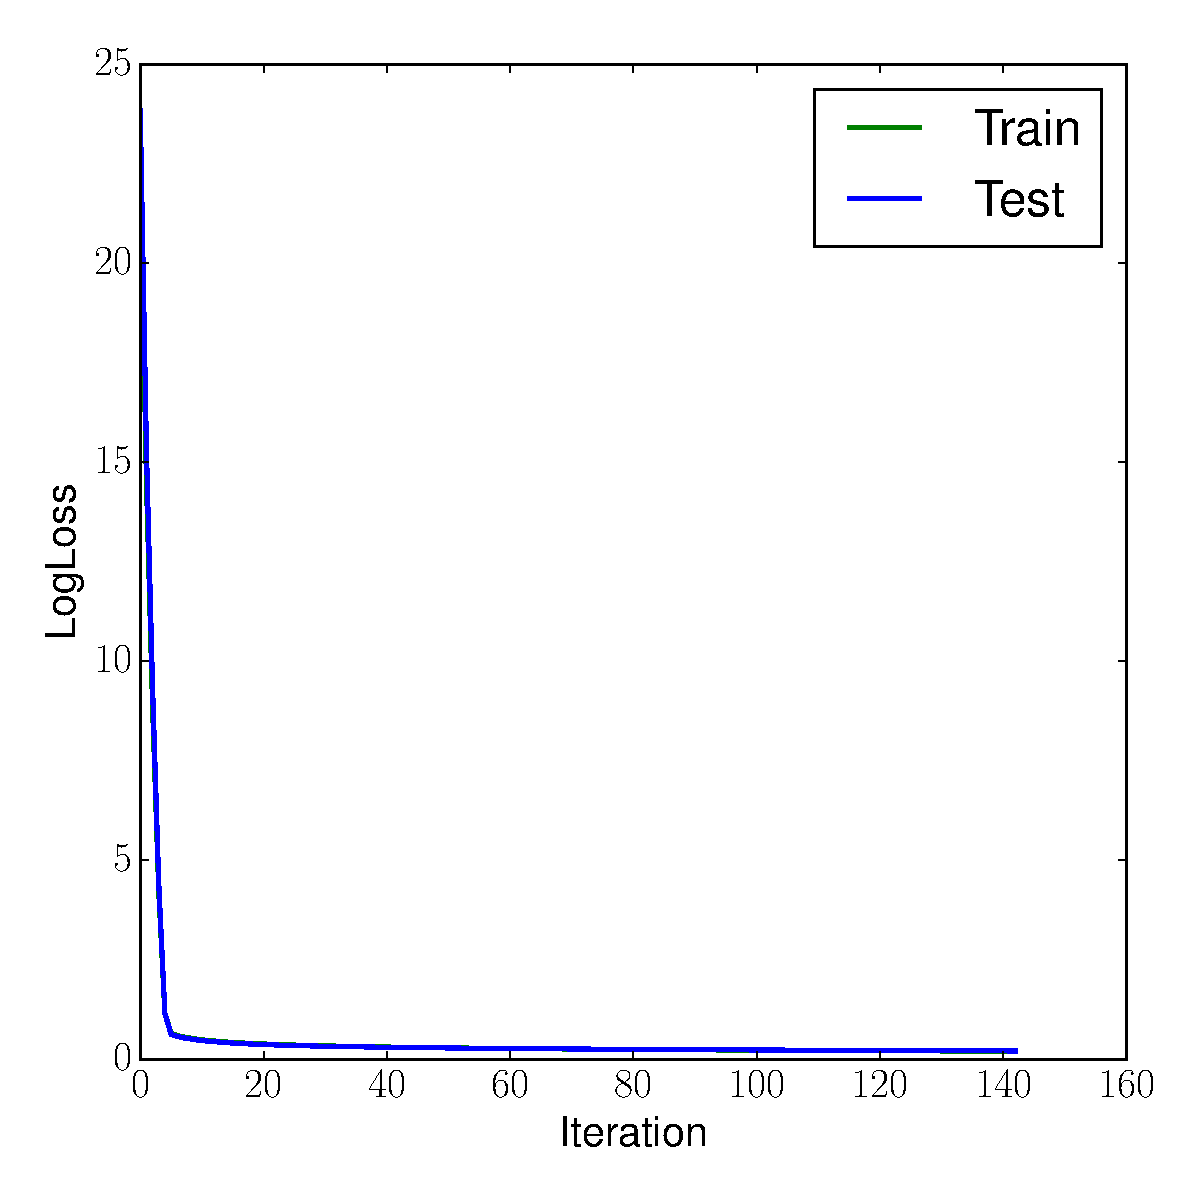
\includegraphics[width=\columnwidth]{mnist_bin_train_test_ll.pdf}
    \caption{Log loss as a function of iteration for both the MNIST training and testing datasets for binary logistic regression.  The log loss on the testing set was evaluated using the model parameters computed by fitting on the training set for each iteration.  The log-losses for both the training and testing sets are very close and hence their evolution appear to overlap in the figure. Note how the loss decreases for both sets with each iteration as the fit improves.  In general, the testing loss is slightly larger than the training loss as expected.}
    \label{fig:mnist_bin_ll}
\end{figure}
\begin{figure}[H]
	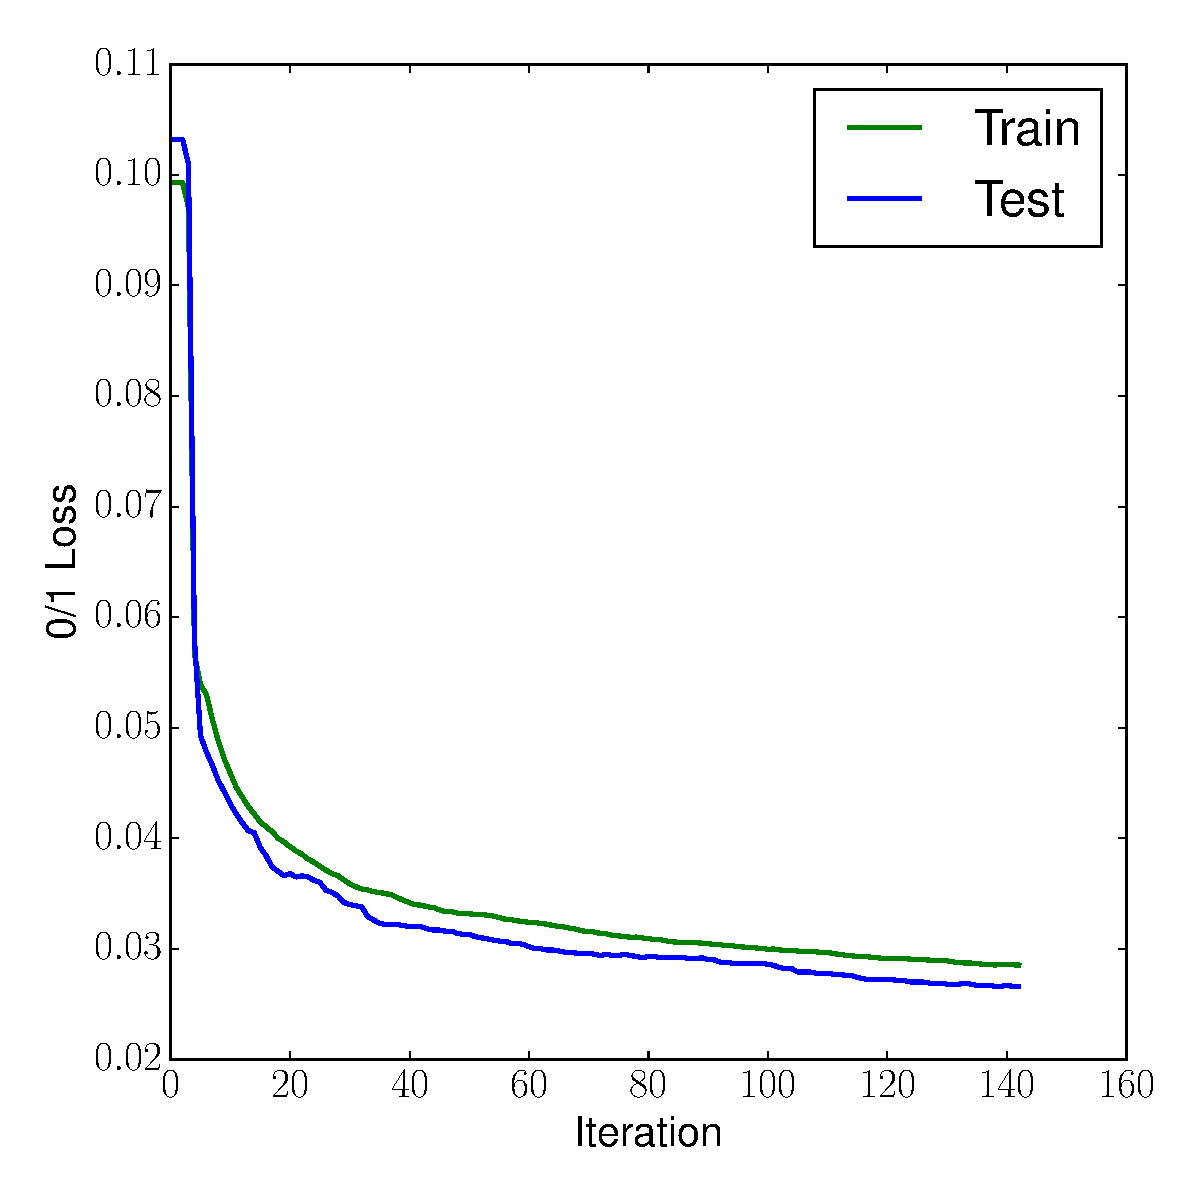
\includegraphics[width=\columnwidth]{mnist_bin_train_test_01.pdf}
    \caption{0/1 loss as a function of iteration for both the MNIST training and testing datasets for binary logistic regression.  The 0/1 loss on the testing set was evaluated using the model parameters computed by fitting on the training set for each iteration.  Note how the loss decreases for both sets with each iteration as the fit improves.  In general, the testing loss is slightly larger than the training loss as expected.}
    \label{fig:mnist_bin_01}
\end{figure}

The log-loss for both sets decreases dramatically during early iterations but then slowly approaches convergence.  The 0/1 loss, on the other hand, does not decrease as dramatically but instead gradually improves until the gradient descent algorithm has convergence.  Once converged, I find my model performs question well and appreciably better than my linear binary classifier from Homework 1 as anticipated.

\subsubsection*{2.1.3}
Given how the sigmoid binary logistic regression link function maps a prediction to a probability-like range $[0,1]$, a natural threshold for classification is to say if $\hat{y} > 0.5$, then $Y = 1$ and 0 otherwise.  With this threshold, I found a training log loss and 0/1 loss of 0.206 and 0.027, respectively.  I found a testing log loss and 0/1 loss of 0.213 and 0.027, respectively.  Note that I normalized both losses by the size of each respective set for comparison's sake.  Overall, my model performs very well at is can successfully classify ${\sim}97\%$ of 2s in the MNIST dataset

\subsection*{2.2: Softmax classification: gradient descent}

In this section I used multi-class softmax classification optimized using batch gradient descent to predict the label of a sample from the MNIST dataset.  For $k$ classes, the labels range over $[0,k-1]$ where for $Y > 0$
\begin{equation} \label{eqn:softmax_p}
P(Y = l | x, w) = \frac{\exp{(w_{0,l} + w^l \cdot x)}}{1 + \sum_{i = 1}^{k-1}\exp{(w_{0,i} + w^i \cdot x)}}
\end{equation}
where I have added a constant offset $w_0$ term for each class for my calculations.  Empirically, I find the model performs slightly better with the inclusion of $w_0$.  For $Y = 0$,
\begin{equation}
P(Y = l | x, w) = \frac{1}{1 + \sum_{i = 1}^{k-1}\exp{(w_{0,i} + w^i \cdot x)}}
\end{equation}
where the probabilities sum to 1.  For classification, I take the largest probability among the coefficients of the prediction vector.  The log-loss for softmax classification is given by 
\begin{equation} \label{eqn:softmax_logloss}
L(w) = \frac{-1}{N} \sum_{i = 1}^N \log(P(Y = y^i | x^i, w))
\end{equation} 
for $N$ samples.  Note that this sum is over the entire prediction vector and not just the predicted probability corresponding to the correct label.  When optimizing my model to find $w_0$ and $\hat{w}$, I seek to minimize Eqn.~\ref{eqn:softmax_logloss}.

\subsubsection*{2.2.1}

Here I take the derivative of the softmax function with respect to $w_p$ for the $lth$ class.  Note that in this case, there are two separate regimes:  where $l = p$ and $l \neq p$ where $l$ is the true class for the $jth$ sample.  Also, I define the indicator function as
\begin{equation} \label{eqn:indicator}
I(y^j, l)
\end{equation}
which returns 1 if $y^j = l$ and 0 otherwise.

First, I expand Eqn.~\ref{eqn:softmax_logloss} and neglect the regularization term for now as it adds a $\lambda w_l$ to the gradient. I find 
\begin{equation} \label{eqn:softmax_logloss_exp}
\begin{split}
NLL & = \sum_j \left[ \log \left[  \frac{\exp{(w_{0,l} + w^l \cdot x^j)}}{1 + \sum_{l = 1}^{k-1}\exp{(w_{0,l} + w^i \cdot x^j)}} \right]\right] \\
& = \sum_j \left[(w_{0,l} + w^l \cdot x^j) - \log[1 + \sum_{l = 1}^{k-1}\exp{(w_{0,l} + w^l \cdot x^j)}] \right]
\end{split}
\end{equation}
via log identities where this quantities is summed over all $j$ samples.

Now, I take the gradient of Eqn.~\ref{eqn:softmax_logloss_exp} for $Y \neq 0$:

\begin{equation} \label{eqn:softmax_grad_neq}
\begin{split}
& \frac{\partial}{\partial w_p} \left( \sum_j \left[(w_{0,l} + w^l \cdot x^j) - \log[1 + \sum_{l= 1}^{k-1}\exp{(w_{0,l} + w^l \cdot x^j)}]\right] \right) \\
& = \sum_j  \sum_{l \neq p} I(y^j = l) \left( \frac{-x^j \exp(w_{0,p} + w_p \cdot x^j)}{1 + \sum_l \exp(w_{0,l} + w_l \cdot x^j)} \right)  \\
& + I(y^j = p) \left( x^j - \frac{x^j \exp(w_{0,p} + w_p \cdot x^j)}{1 + \sum_l \exp(w_{0,l} + w_l \cdot x^j)} \right)
\end{split}
\end{equation}
where the two terms account for cases when the true label $l \neq p$ and when $l = p$ where $p$ is the current class whose derivative I evaluate.  Replacing terms with conditional probabilities yield
\begin{equation}
\sum_j \sum_{l \neq p} -I(y^j = l) x^j P(y^j = p | x^j, w) + I(y^j = p) x^j \left[1 - P(y^j = p | x^j, w) \right]
\end{equation}
which is similar to the binary logistic regression case but with additional terms for all incorrectly labeled terms in the prediction vector.

Now the gradient for the $Y = 0$ term proceeds similarly but without the $w_{0,l} + w^l \cdot x^j$ term as goes as follows: 

\begin{equation} \label{eqn:softmax_grad_eq}
\begin{split}
& \frac{\partial}{\partial w_p} \left( \sum_j \left[- \log[1 + \sum_{l= 1}^{k-1}\exp{(w_{0,l} + w^l \cdot x^j)}]\right] \right) \\
& = \sum_j  \sum_{l \neq p} I(y^j = l) \left( \frac{-x^j \exp(w_{0,p} + w_p \cdot x^j)}{1 + \sum_l \exp(w_{0,l} + w_l \cdot x^j)} \right)  \\
& + I(y^j = p) \left( - \frac{x^j \exp(w_{0,p} + w_p \cdot x^j)}{1 + \sum_l \exp(w_{0,l} + w_l \cdot x^j)} \right).
\end{split}
\end{equation}
Replacing with conditional probabilities and simplifying gives
\begin{equation}
\sum_j \sum_{l \neq p} -I(y^j = l) x^j P(y^j = p | x^j, w) + I(y^j = p) x^j \left[- P(y^j = p | x^j, w) \right]
\end{equation}

The gradient derived above becomes the gradient for my regularized gradient descent update rule
\begin{equation}
 w_l^{(t+1)} \leftarrow w_l^{(t)} - \eta (\lambda w_l^{(t)} + \nabla_l NLL(w_l)).
 \end{equation}
 In practice, I convert my $n \times 1$ label vector $y$ into $n \times k$ label matrix for $k$ classes.  For the $jth$ sample $y_j$, the element corresponding to the correct label is 1 while all other elements are 0.  Naturally, my $w$ becomes a $d \times k$ matrix and $w_0$ becomes a $k \times 1$ vector.  Inserting my derived gradients into the gradient descent update rule, I update $w$ and $w_0$ as follows
 
 \begin{equation}
w^{(t+1)}_l \leftarrow w^{(t)}_l - \eta (\lambda w^{(t)}_l - \sum_j x^j_i[y^j - \hat{P}(Y^j = l | x^j, w_l^{(t)})])
\end{equation}
and for the unregularized constant offset term
\begin{equation}
w^{(t+1)}_{0,l} \leftarrow w^{(t)}_{0,l} - \eta (- \sum_j[y^j - \hat{P}(Y^j = l | x^j, w^{(t)})]).
\end{equation}
where these expressions can simultaneously be evaluated for all $l$ when both $w$ and $y$ are converted into matrices as described above.

For my implementation, I found it easier to solve the over-constrained softmax
\begin{equation}
P(Y = l | x, w) = \frac{\exp{(w_{0,l} + w^l \cdot x)}}{\sum_{i = 1}^{k}\exp{(w_{0,i} + w^i \cdot x)}}
\end{equation}
where I also fit for a $w_0$ and a $w$ for the $Y = 0$ term.  I found that this version of softmax was more intuitive to interpret and yielded reasonable results when combined with $l_2$ regularization.  In this formalism, the negative log-likelihood, log-loss, becomes

\begin{equation} \label{eqn:softmax_logloss_exp_actual}
\begin{split}
NLL & = \sum_j \left[ \log \left[  \frac{\exp{(w_{0,l} + w^l \cdot x^j)}}{\sum_{l = 1}^{k}\exp{(w_{0,l} + w^i \cdot x^j)}} \right]\right] \\
& = \sum_j \left[(w_{0,l} + w^l \cdot x^j) - \log[\sum_{l = 1}^{k}\exp{(w_{0,l} + w^l \cdot x^j)}] \right].
\end{split}
\end{equation}

I took the derivative of this term to get my gradient term for my update rule.  The math proceeds just as above for the $Y \neq 0$ case but without the normalizing 1 in the denominator to again yield
\begin{equation}
\sum_j \sum_{l \neq p} -I(y^j = l) x^j P(y^j = p | x^j, w) + I(y^j = p) x^j \left[- P(y^j = p | x^j, w) \right]
\end{equation}
in terms on conditional probabilities.  When I fold in a $l_2$ regularization term, the update rules become
 \begin{equation}
w^{(t+1)}_l \leftarrow w^{(t)}_l - \eta (\lambda w^{(t)}_l - \sum_j x^j_i[y^j - \hat{P}(Y^j = l | x^j, w_l^{(t)})])
\end{equation}
and for the unregularized constant offset term
\begin{equation}
w^{(t+1)}_{0,l} \leftarrow w^{(t)}_{0,l} - \eta (- \sum_j[y^j - \hat{P}(Y^j = l | x^j, w^{(t)})]).
\end{equation}
as before.  These are the update rules I implemented to solve the softmax classification problem using gradient descent (see the function {\tt multi$\_$logistic$\_$grad} in the file {\tt classifier$\_$utils.py}).

\subsubsection*{2.2.2}

For my regularized batch gradient descent implementation, I used the $l_2$ norm penalty.  When fitting this algorithm, I need to optimize of the following hyperparameters: the learning rate $\eta$ and the regularization constant $\lambda$.  The hyperparameters of my model were simultaneously fit for along a regularization grid.  Since my training set was sufficiently large with $N = 60,000$ samples, I randomly partitioned it into a validation set with $N_{val} = 6,000$ and a training set with $N_{train} = 54,000$.  I iterated over a two-dimensional grid of $\eta \in [10^{-7},10^{-3}]$ in 5 logarithmic bins and $\lambda \in [10^{-2},10^{3}]$ in 5 logarithmic bins.  For each $(\eta,\lambda)$ pair, I ran batch gradient descent on the training set then tested it on the validation data.  I used the validation predictions to compute the 0/1 loss and stored it for each grid point.  I found the optimal learning rate $\eta = 10^{-4}$ and $\lambda = 10^3$ from the minimum value of the 0/1 loss grid.  

\subsubsection*{2.2.3}

In Fig.~\ref{fig:bgd_mnist_ll} and Fig.~\ref{fig:bgd_mnist_01}, I plot the log-loss and 0/1 loss as a function of iteration for my softmax logistic regression batch gradient descent solution.  Initially in the first two or so iterations, my solution moves away from the local minimum, likely because the initial step size $\eta$ was a bit too large.  As the iteration number increased and $eta$ decayed as $1/\sqrt{t}$ for iteration number $t$, the decreased step size allowed the algorithm to advance towards to local minimum.  Eventually around iteration 15, the solution reached close to the local minimum and slowly converged from there.  Note that for this question, I said my solution was converged once the log-loss changed by less than $0.5\%$ between iterations.  A stricter converged criterion did not appreciably improve final losses and only slowed down the code.  Interestingly, I found lower losses on my testing set indicated that my model performed marginally better on my testing set than the training set.

\begin{figure}[H]
	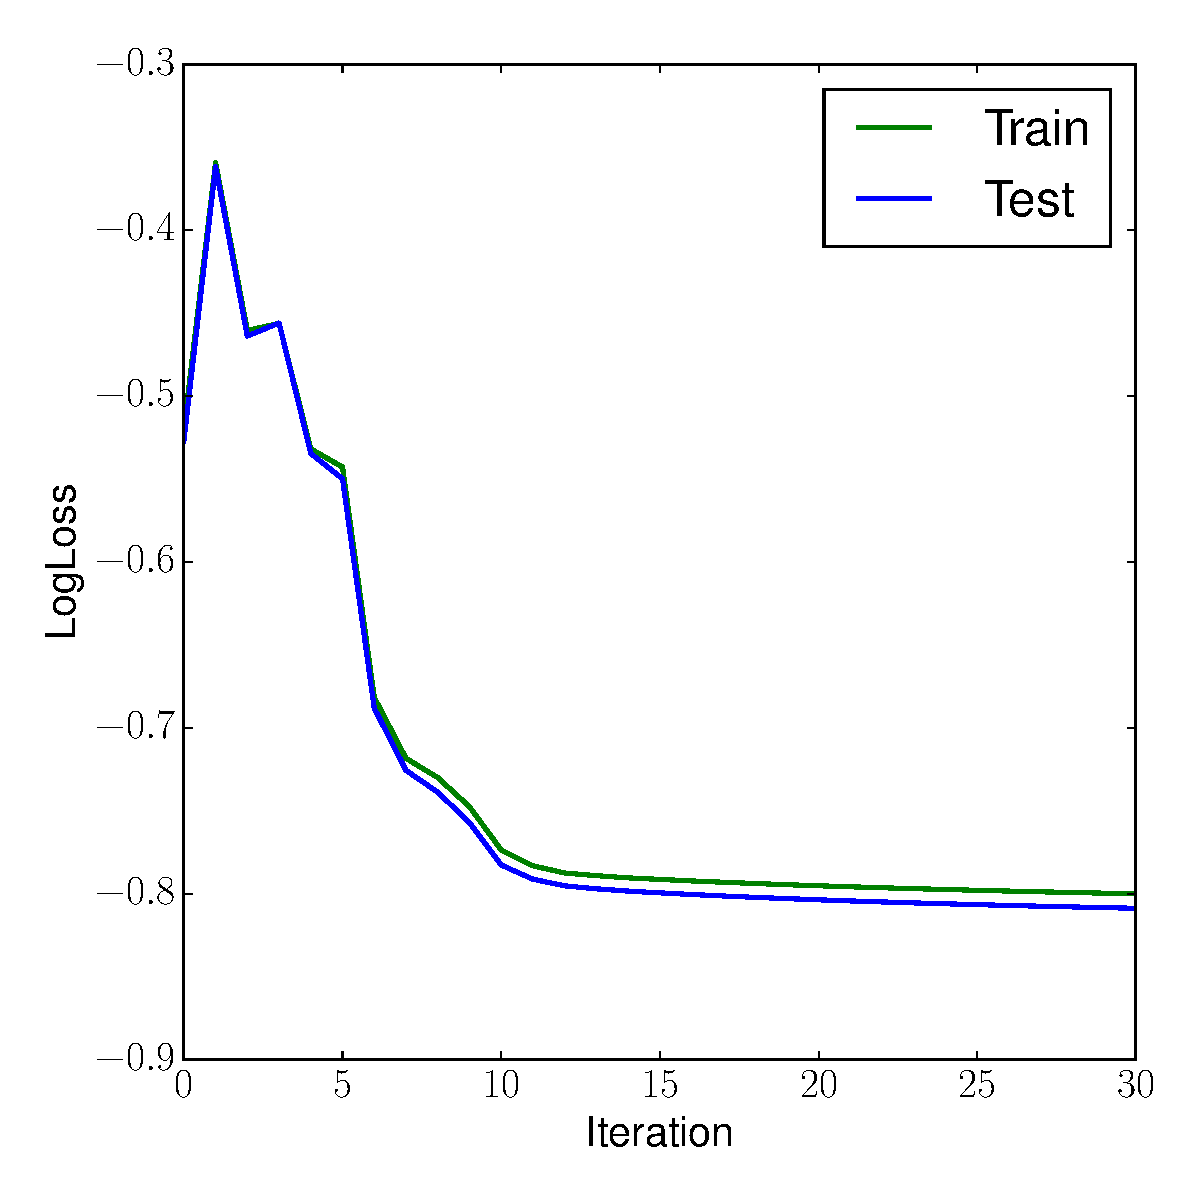
\includegraphics[width=\columnwidth]{bgd_mnist_multi_train_test_ll.pdf}
    \caption{Log loss as a function of iteration for both the MNIST training and testing datasets for softmax logistic regression using batch gradient descent.  The log loss on the testing set was evaluated using the model parameters computed by fitting on the training set for each iteration.  The log-losses for both the training and testing sets are very close and hence their evolution appear to overlap in the figure.  Note how the loss decreases for both sets with each iteration as the fit improves.}
    \label{fig:bgd_mnist_ll}
\end{figure}
\begin{figure}[H]
	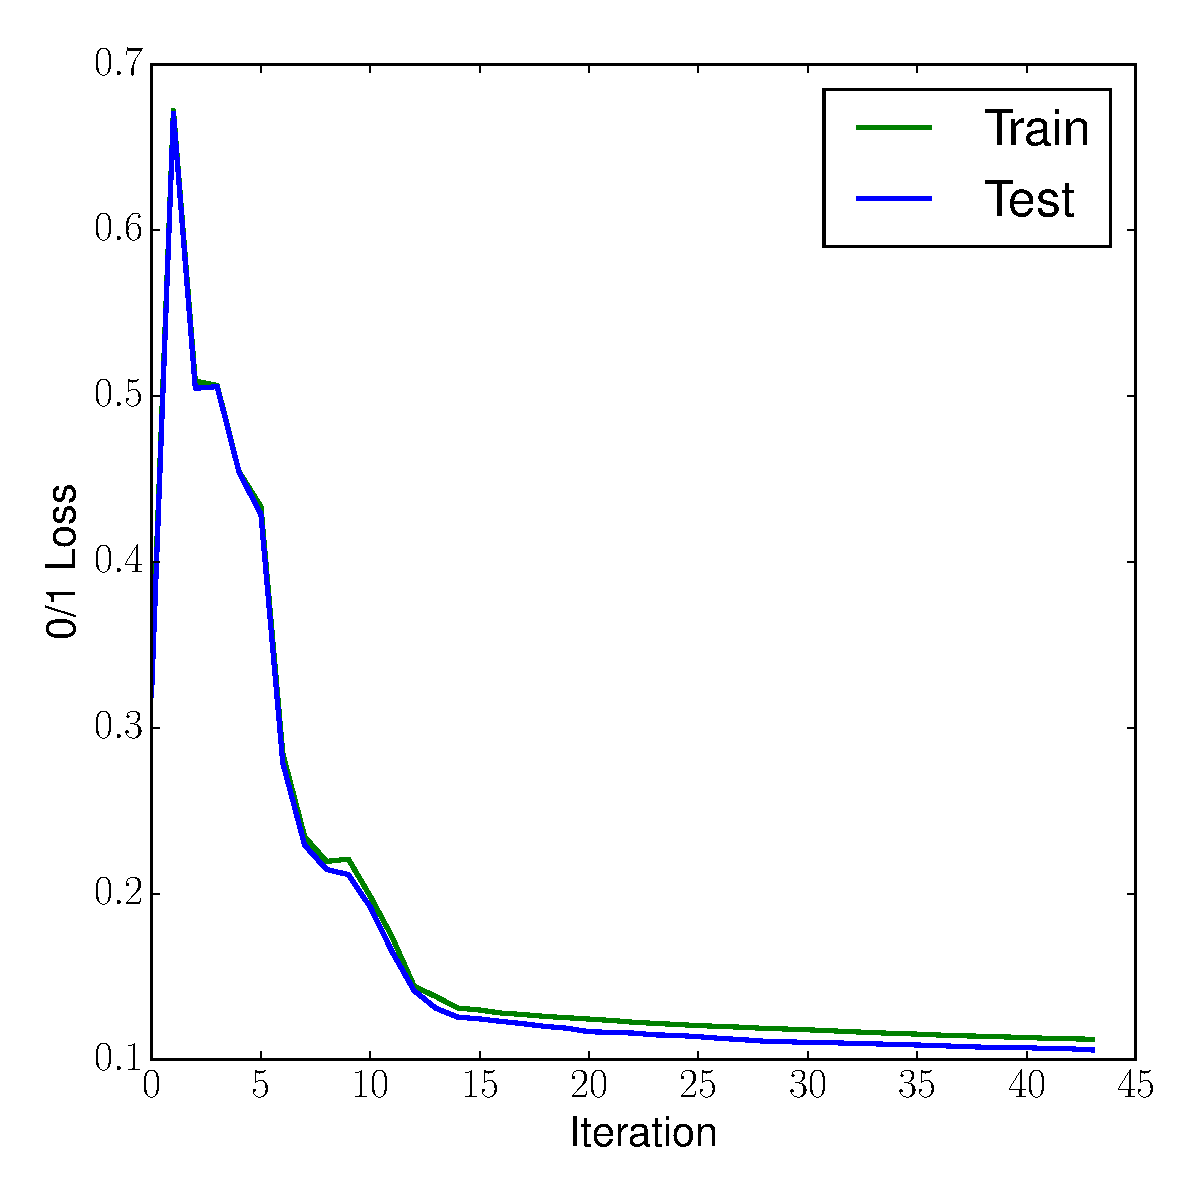
\includegraphics[width=\columnwidth]{bgd_mnist_multi_train_test_01.pdf}
    \caption{0/1 loss as a function of iteration for both the MNIST training and testing datasets for softmax logistic regression using batch gradient descent.  The 0/1 loss on the testing set was evaluated using the model parameters computed by fitting on the training set for each iteration.  Note how the loss decreases for both sets with each iteration as the fit improves.}
    \label{fig:bgd_mnist_01}
\end{figure}

\subsubsection*{2.2.4}

On the training set, I achieved a log-loss and a 0/1 loss of 0.439 and 0.112, respectively.  On the testing set, I achieved a final log-loss and a 0/1 loss of 0.419, 0.106, respectively.  My simple batch gradient descent solution for softmax logistic regression performs rather well as it can correctly classify ${\sim}90\%$ of digits in the MNIST dataset.

\subsection*{2.3: Softmax classification: stochastic gradient descent}

In this section, I again optimize my softmax logistic classifier but this time I use stochastic gradient descent (SGD).  My SGD implementation is located in {\tt DML/optimization/gradient$\_$descent.py} in the {\tt stochastic$\_$gradient$\_$descent} function.  For my implementation, I allowed the user to specify a particular batch size where 1 corresponds to regular SGD and $> 1$ is minibatch SGD.  The code used to answer this question and all subquestions are contained within the following python files: {\tt hw2$\_$2.3.py} in the {\tt HW2} directory and {\tt classification/classifier$\_$utils.py, validation/validation.py, data$\_$processing/mnist$\_$utils.py, gradient$\_$descent/gradient$\_$descent.py} in the {\tt DML} directory.

In my implementation, I define an epoch as each complete pass through the training set.  At the start of each epoch, I randomly shuffle my training set and partition it into batches based on the batch size.  I then loop over all batches where I update $w$ and $w_0$ according to the gradient computing using just that batch as opposed to the gradient computing using the entire training set as is done in batch gradient descent.  As suggested in the homework prompt, I define an iteration as each pass through the training set.  Each iteration, I compute and store various loss metrics for subsequent analysis.  In addition, I check for convergence after each iteration.  I say my solution has converged once my log-loss changes by less than $0.5\%$.  I find that small convergence criteria do little to improve my results.  I decrease my learning rate using the same procedure outlined above in the discussion of my batch gradient descent implementation.

\subsubsection*{2.3.1}

I implemented SGD using a minibatch size of 1.  As discussed above, I computed the log-loss and the 0/1 loss after each iteration where an iteration is defined as a pass through 15,000 samples.  I found a learning rate $\eta = 5 \times 10^{-6}$ yielded good performance and convergence.  Using Eqn.~\ref{eqn:lambda_heuristic}, I found a regularization parameter of $\lambda = 1$ yielded the best performance.  In Fig.~\ref{fig:sgd_mnist_ll} and Fig.~\ref{fig:sgd_mnist_01} I plot the log-loss and 0/1 loss as a function of iteration for my softmax classification using SGD.  In both figures, I plot a horizontal line representing the respective loss values computed by applying the converged batch gradient descent softmax classification model on the MNIST testing set for reference.

\begin{figure}[H]
	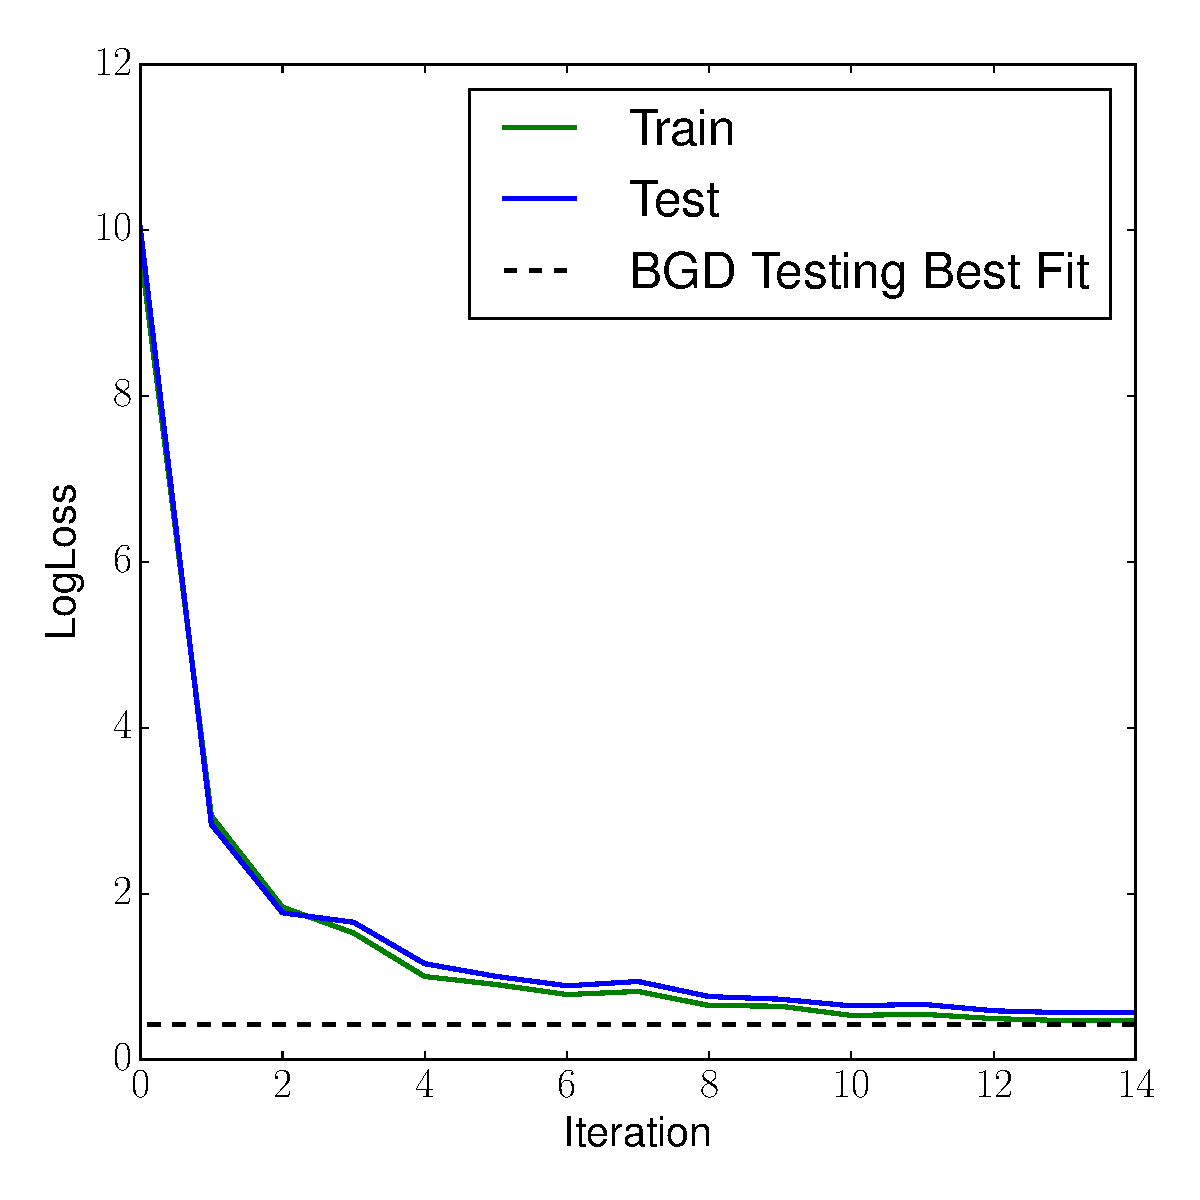
\includegraphics[width=\columnwidth]{sgd_mnist_multi_train_test_ll.pdf}
    \caption{Log loss as a function of iteration for both the MNIST training and testing datasets for softmax logistic regression using SGD.  The log loss on the testing set was evaluated using the model parameters computed by fitting on the training set for each iteration.  The testing set loss is always greater than the training set loss as expected.}
    \label{fig:sgd_mnist_ll}
\end{figure}
\begin{figure}[H]
	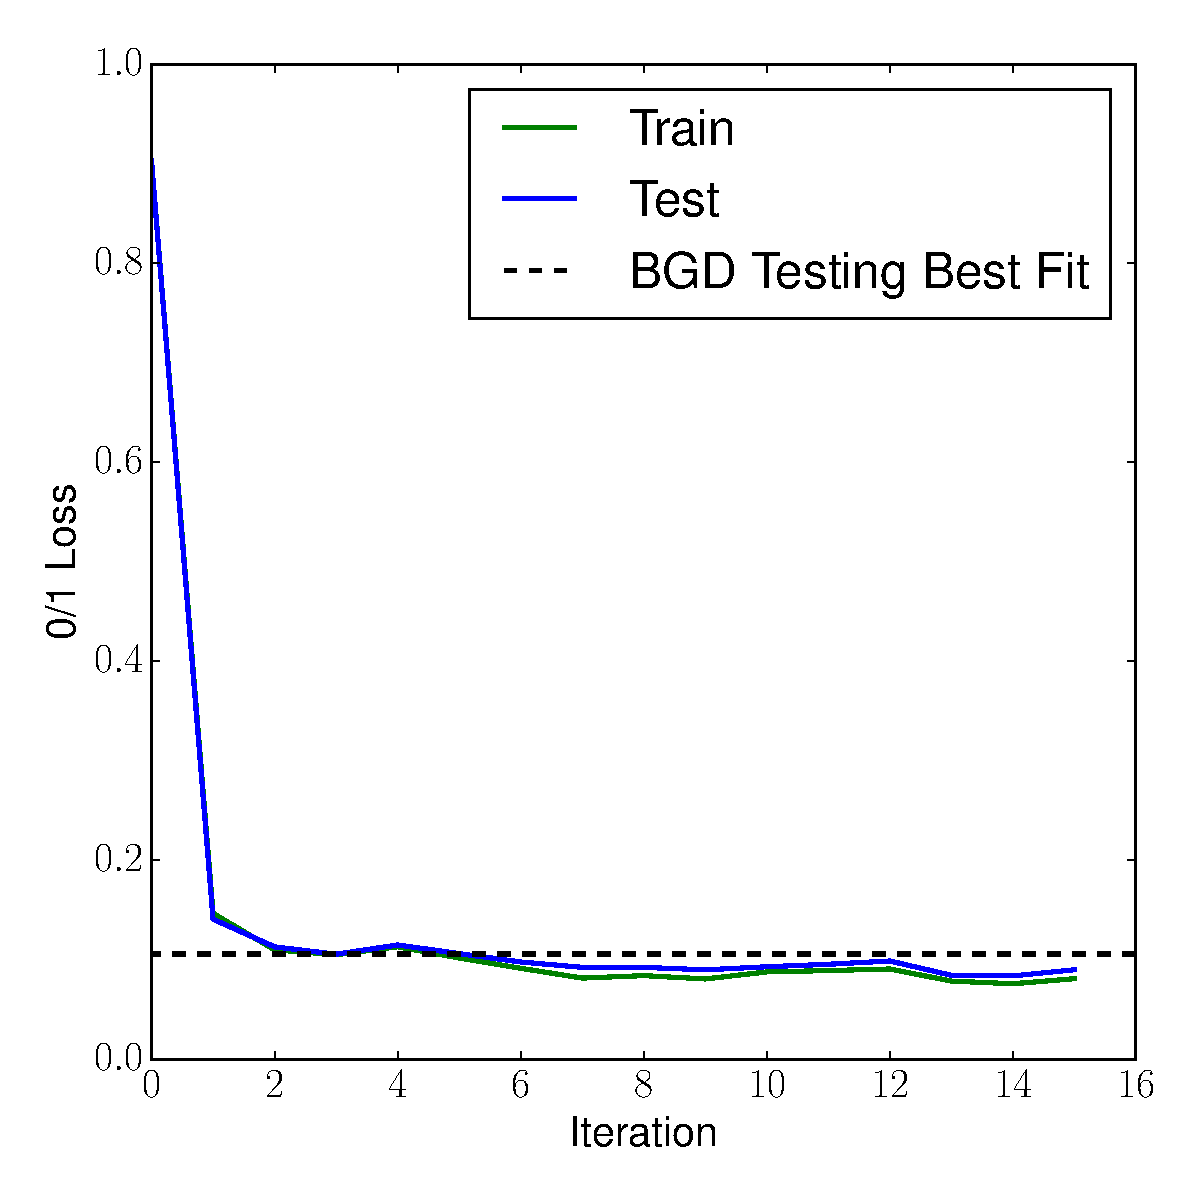
\includegraphics[width=\columnwidth]{sgd_mnist_multi_train_test_01.pdf}
    \caption{0/1 loss as a function of iteration for both the MNIST training and testing datasets for softmax logistic regression using SGD.  The 0/1 loss on the testing set was evaluated using the model parameters computed by fitting on the training set for each iteration.  Both 0/1 losses rapidly achieve comparable performance to the batch gradient descent optimized case.}
    \label{fig:sgd_mnist_01}
\end{figure}

As seen in both figures, the losses rapidly drop to the performance of the batch gradient descent optimized problem.  Interestingly, it takes the log-loss about 12 iterations to achieve similar performance to the batch gradient descent optimized case while it takes about 4 for the 0/1 loss.  This indicated that even though the SGD is approaching closer to the minimum, it is not appreciably improving the softmax's ability to classify the MNIST digits.  I do note, however, that the SGD optimized case achieves a better 0/1 loss than the batch gradient descent case.  The SGD achieved a training set log-loss and 0/1 loss of 0.379 and 0.081 while achieving a log-loss and 0/1 loss of 0.453 and 0.09 on the testing set, respectively.  As stated previously, I used a learning rate of $\eta = 5 \times 10^{-6}$ and decayed $\eta$ as $1/\sqrt{t}$ where $t$ is the number of the current iteration.

\subsubsection*{2.3.2}

My SGD implementation converged to a better solution in terms of 0/1 loss than my batch gradient descent solution much more quickly.  For example, it took 42 passes through the training set for batch gradient descent to converge to an 0/1 loss of about 0.1 while my SGD implementation took only 1 pass through the training set to achieve the same 0/1 loss!  My SGD implementation took about 3 passes through the training set to achieve a similar log-loss and my batch gradient descent implementation.  This speed-up is rather impressive and suggests that the gradient is rather well-behaved in the MNIST data as gradients computed from random samples from the training set still led the solution in the proper direction.

\subsubsection*{2.3.3}

I implemented mini-batch SGD using a batch size of 100 samples.  In Fig.~\ref{fig:sgd_mini_mnist_ll} and Fig.~\ref{fig:sgd_mini_mnist_01} I plot the log-loss and 0/1 loss as a function of iteration for my softmax classification using SGD.  In both figures, I plot a horizontal line representing the respective loss values computed by applying the converged batch gradient descent softmax classification model on the MNIST testing set for reference.

\begin{figure}[H]
	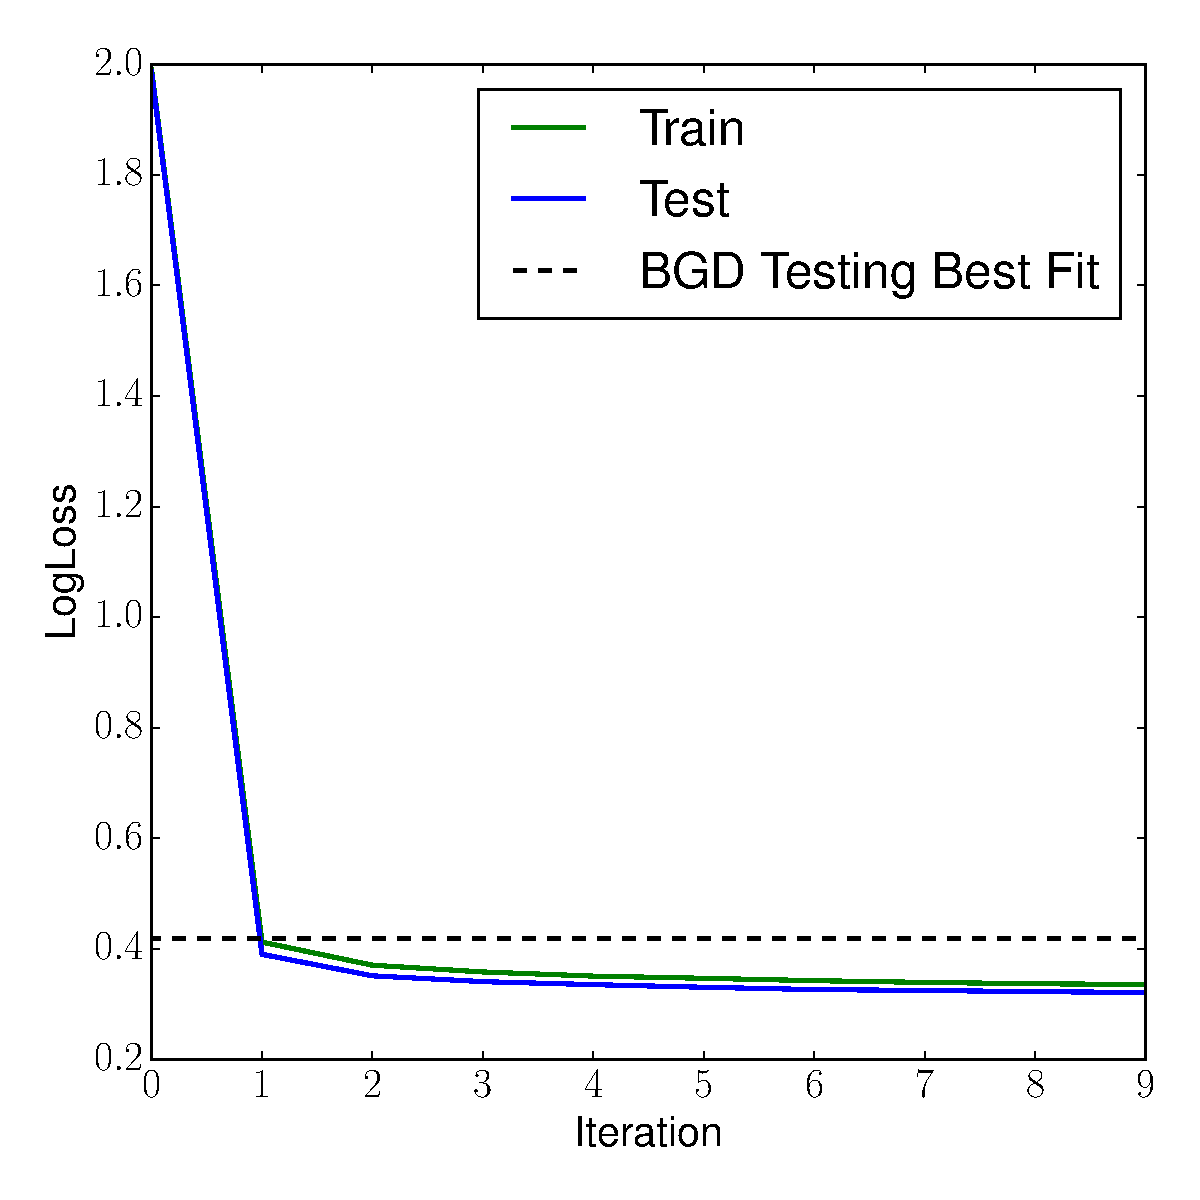
\includegraphics[width=\columnwidth]{sgd_mini_mnist_multi_train_test_ll.pdf}
    \caption{Log loss as a function of iteration for both the MNIST training and testing datasets for softmax logistic regression using mini-batch SGD.  The log loss on the testing set was evaluated using the model parameters computed by fitting on the training set for each iteration.  The testing set loss is always greater than the training set loss as expected.}
    \label{fig:sgd_mini_mnist_ll}
\end{figure}
\begin{figure}[H]
	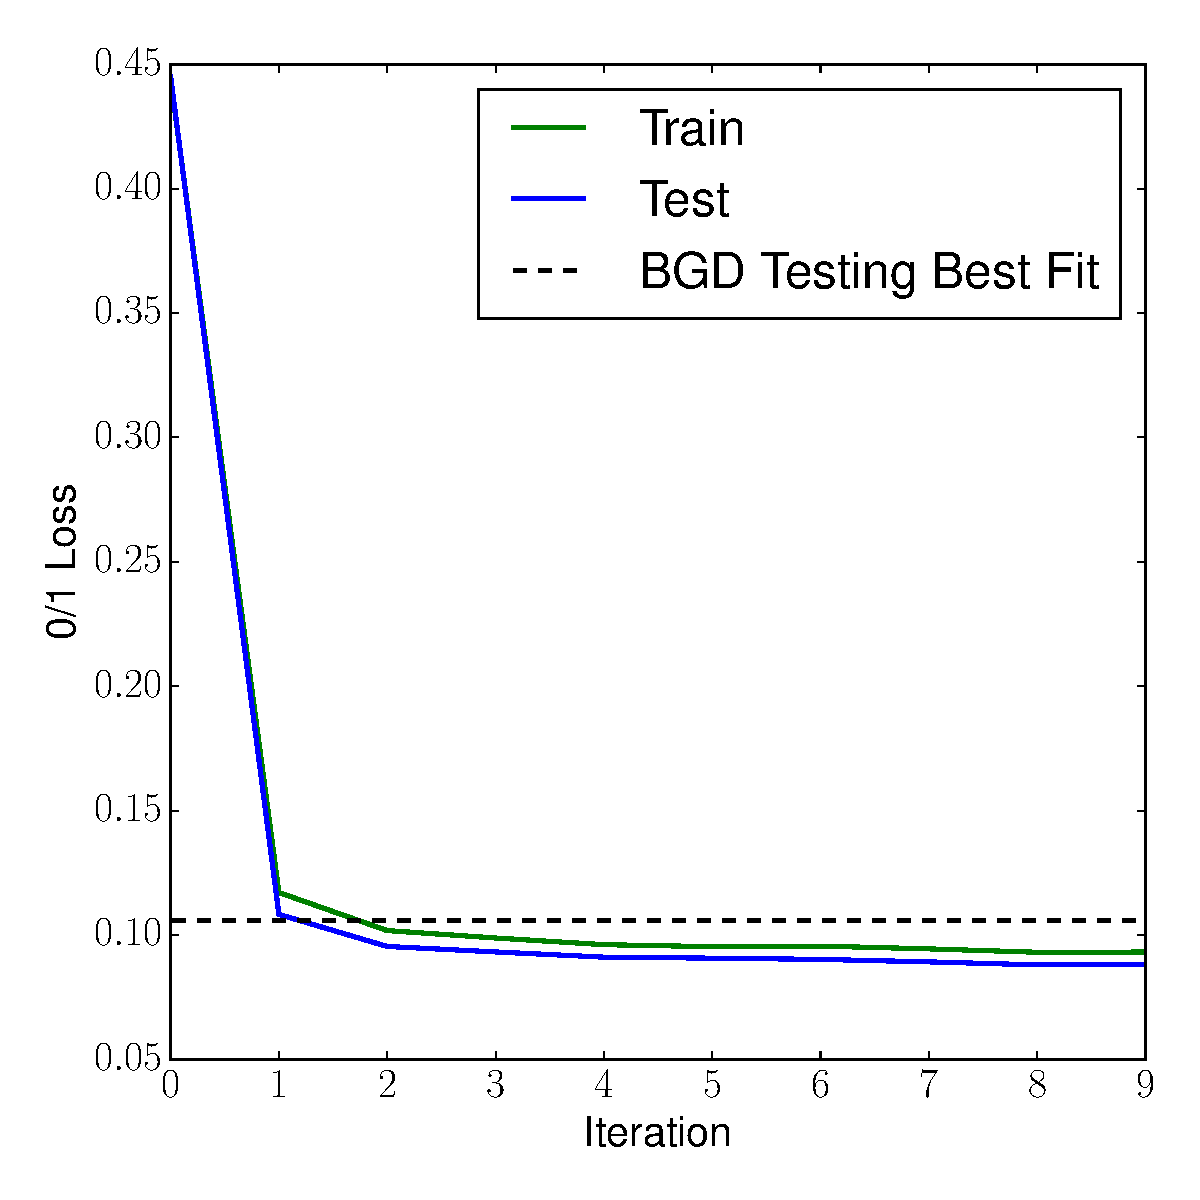
\includegraphics[width=\columnwidth]{sgd_mini_mnist_multi_train_test_01.pdf}
    \caption{0/1 loss as a function of iteration for both the MNIST training and testing datasets for softmax logistic regression using mini-batch SGD.  The 0/1 loss on the testing set was evaluated using the model parameters computed by fitting on the training set for each iteration.  Both 0/1 losses rapidly achieve comparable performance to the batch gradient descent optimized case.}
    \label{fig:sgd_mini_mnist_01}
\end{figure}

As seen in both figures, the losses immediately drop to the batch gradient descent performance after 1 iteration, or 150 batches through 15,000 samples!  After several more iterations, my mini-batch SGD algorithm converged to performance that was markedly better than the batch gradient descent implementation.  The mini-batch SGD achieved a training set log-loss and 0/1 loss of 0.341 and 0.095 while achieving a log-loss and 0/1 loss of 0.326 and 0.09 on the testing set, respectively.

After trial and error, I found that a learning rate $\eta = 5 \times 10^{-6}$ gave the best performance.  Any larger learning rate caused the algorithm to diverge.  As before, I decayed $\eta$ as $1/\sqrt{t}$ where $t$ is the number of the current iteration.  Using Eqn.~\ref{eqn:lambda_heuristic}, I found a regularization parameter of $\lambda = 1$ yielded the best performance.

\subsubsection*{2.3.4}

My mini-batch algorithm converged more quickly than my SGD algorithm at 1 iteration to reach batch gradient descent performance as compared to over 4 for SGD.  Mini-batch SGD only needed to pass through about one quarter of the training data before achieving batch gradient descent performance while it took vanilla SGD at least one full pass through all 60,000 points.  This is likely due to the inherent noise incurred from computing the gradient with one data point as is done with SGD causing the solution to bounce around more as opposed to a smooth decent to the minimum.  In mini-batch SGD, computing the gradient over 100 samples smooths out the noise to result in a quicker convergence down towards the minimum.

\subsection*{2.4: Neural Nets with a random first layer: Using more features}

The code used to solve this question is in the following attached files: {\tt hw2$\_$2.4.py} in the {\tt HW2} directory and {\tt classification/classifier$\_$utils.py, regression/regression$\_$utils.py, validation/validation.py, data$\_$processing/mnist$\_$utils.py}, 
{\tt gradient$\_$descent/gradient$\_$descent.py} in the {\tt DML} directory.

\subsubsection*{2.4.1}

For this question, I transformed my MNIST image datasets using the same transformation matrix $v$ I used in Question 1.2 for consistency.  Given the size of the transformed data ($60000 \times 10000$) and also the convergence speeds analyzed in the previous question, I decided to using mini-batch SGD to optimized a softmax classifier on this data.  After trial and error, error being where my solution diverged, I found a learning rate $\eta = 1 \times 10^{-8}$ yielded the best performance.  Using Eqn.~\ref{eqn:lambda_heuristic}, I found a regularization parameter of $\lambda = 2.8 \times 10^{4}$ yielded the best performance.  As before, I deem my algorithm converged once the log-loss changes by less than $0.5\%$ and for SGD, each pass through 15,000 samples is referred to as an iteration.

In Fig.~\ref{fig:sgd_nn_mini_mnist_ll} and Fig.~\ref{fig:sgd_nn_mini_mnist_01} I plot the log-loss and 0/1 loss as a function of iteration for my softmax classification using mini-batch SGD on the transformed MNIST data.  In both figures, I plot a horizontal line representing the respective loss values computed by applying the converged batch gradient descent softmax classification model on the MNIST testing set for reference.

\begin{figure}[H]
	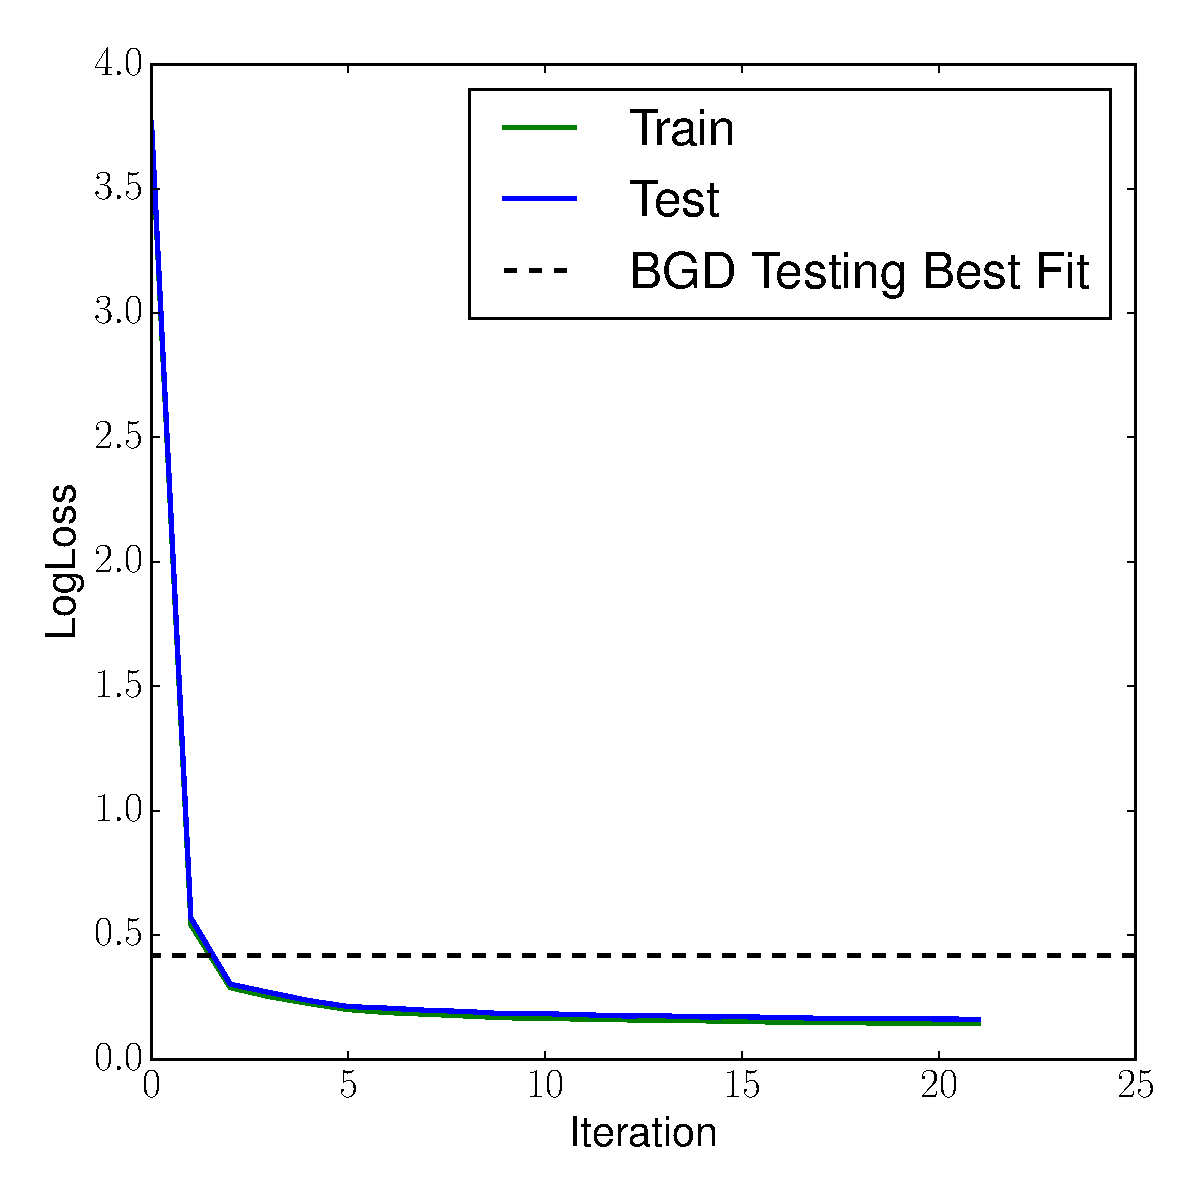
\includegraphics[width=\columnwidth]{sgd_nn_mnist_multi_train_test_ll.pdf}
    \caption{Log loss as a function of iteration for both the transformed MNIST training and testing datasets for softmax logistic regression using mini-batch SGD.  The log loss on the testing set was evaluated using the model parameters computed by fitting on the training set for each iteration.}
    \label{fig:sgd_nn_mini_mnist_ll}
\end{figure}
\begin{figure}[H]
	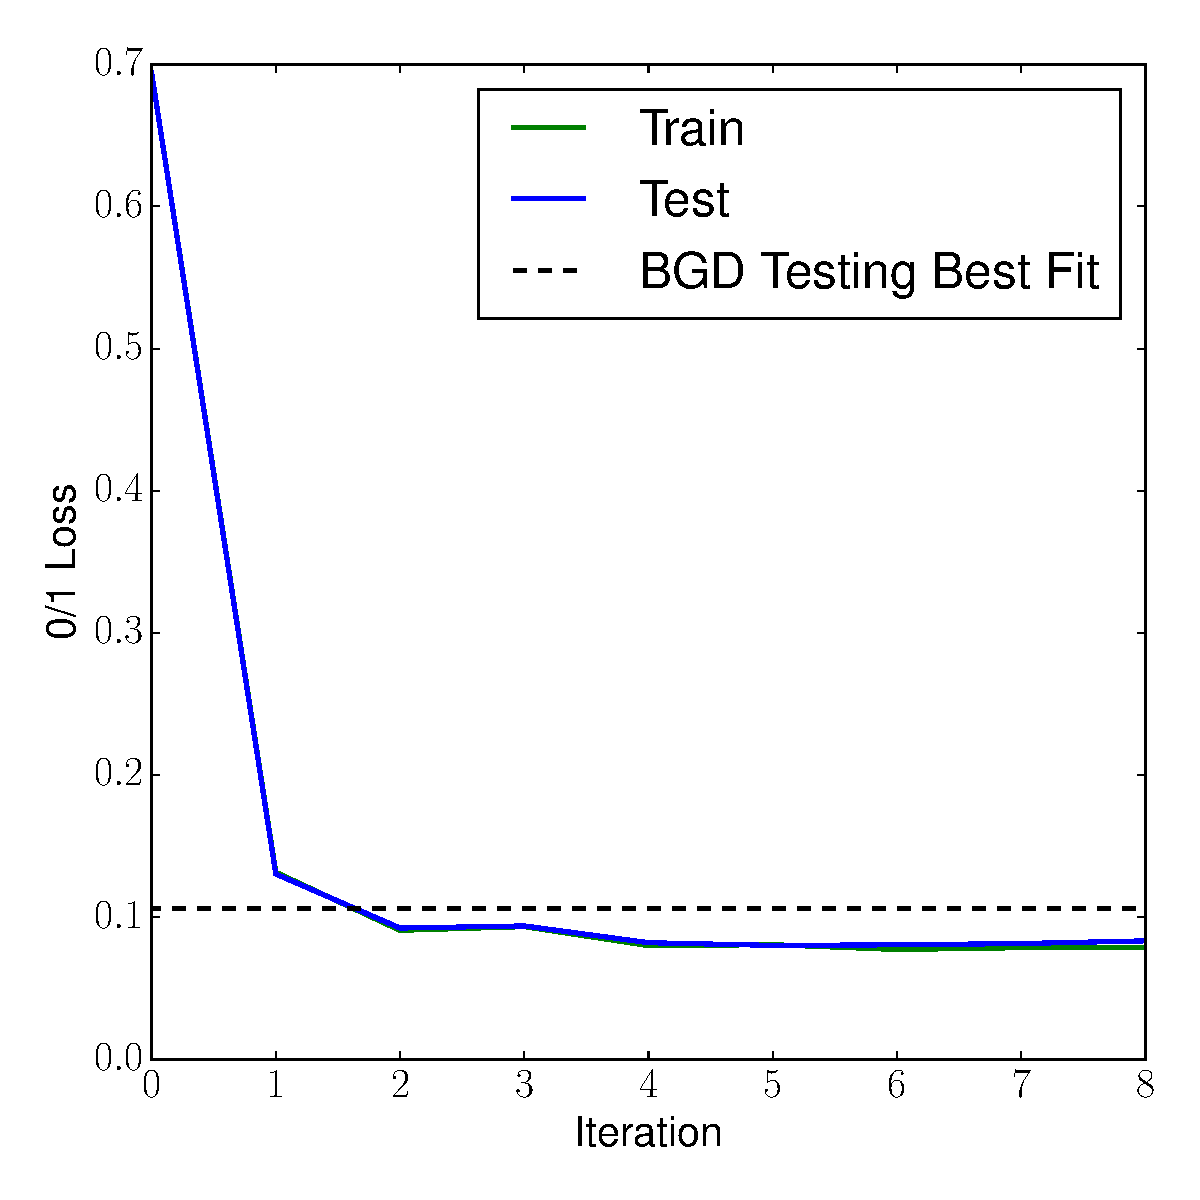
\includegraphics[width=\columnwidth]{sgd_nn_mnist_multi_train_test_01.pdf}
    \caption{0/1 loss as a function of iteration for both the transformed MNIST training and testing datasets for softmax logistic regression using mini-batch SGD.  The 0/1 loss on the testing set was evaluated using the model parameters computed by fitting on the training set for each iteration.}
    \label{fig:sgd_nn_mini_mnist_01}
\end{figure}

As seen above, the mini-batch SGD quickly achieves performance comparable to the gradient descent softmax optimization on the original MNIST data after only 2 iterations, or just half a pass through the training set.  The losses for both the training and testing set as a function of iteration are nearly identical until the algorithm finally converges at which point the testing loss is slightly greater than the training loss.

\subsubsection*{2.4.2}

The mini-batch SGD on the transformed MNIST data achieved a training set log-loss and 0/1 loss of 0.144 and 0.040 while achieving a log-loss and 0/1 loss of 0.162 and 0.047 on the testing set, respectively.  As expected, the testing loss is greater than the training loss.  Interestingly, both the log and 0/1 losses on the transformed data are appreciably smaller than their counter-parts on the original MNIST data.  Even though I used the same optimization algorithm, mini-batch SGD, and softmax classification, the one layer neural network transformed MNIST data yields a markedly better performance than the original data.  Even though I did nothing particularly clever when transforming the MNIST data to a space with more features, this trivial step yielded non-trivial improvements.

\section*{3: (Baby) Learning Theory: Why is statistical learning possible?}

For this question, I will assume a simplified Chernoff-Hoeffding bound of the following form
\begin{equation} \label{eqn:ch_bound}
P(|\bar{Z} - \theta| \geq \epsilon) \leq 2 \exp(-2N \epsilon^2)
\end{equation}
where $\bar{Z}$ is the empirical mean of N i.i.d. samples from a Bernoulli distribution where $P(Z = 1) = \theta$ and $P(Z = 0) = 1 - \theta$.  Additionally, I will be working in the hypothesis space where I have a finite set of $K$ classifiers.  For this Question, I want to note a few things that I will use in subsequent proofs.  The quantity $\bar{Z}$ is an empirical quantity learned from the respective training set $T$ whereas $\theta$ is the expected value for $\bar{Z}$ over the underlying distribution like the bias of a coin the expected value of the MLE for the Bernoulli distribution and as such the MLE is unbiased.  I use these facts to relate quantities to both $\bar{Z}$ and $\theta$ to show when the Chernoff-Hoeffding bound applies.  This is especially relevant since in this question, I work with 0/1 loss where the 0/1 loss on each sample can be considered an i.i.d. sample from a Bernoulli distribution.

\subsection*{3.1: A confidence interval for a coin}

\subsubsection*{3.1.1}

A confidence interval for the quantities $|\bar{Z} - \theta|$ is for the probability of that quantity being smaller than some error threshold $\epsilon$ to be something like $95\%$ in which case $1 - \delta = 0.95$ for $\delta = 0.5$.  To quantify the confidence interval, I seek to derive a functional form for $\epsilon$ in terms of $N$ and $\delta$.

\begin{equation}
\begin{split}
& P(|\bar{Z} - \theta| \leq \epsilon) \geq 1 - \delta \\
& P(|\bar{Z} - \theta| \leq \epsilon) - 1 \geq - \delta \\
& 1- P(|\bar{Z} - \theta| \leq \epsilon) \leq \delta \\
& P(|\bar{Z} - \theta| \geq \epsilon) \leq \delta
\end{split}
\end{equation}
via the law of total probability.  At this point, I note that the final expression is equivalent in form to Eqn.~\ref{eqn:ch_bound} and therefore I can equate
\begin{equation}
\delta = 2 \exp(-2N \epsilon^2).
\end{equation}
With this expression in hand, I can solve for $\epsilon$ and complete the confidence interval derivation as follows:
\begin{equation} \label{eqn:eps_bound}
\begin{split}
& \log (\delta/2) = \log(\exp(-2N \epsilon^2)) \\
& \log(\delta/2) -2N \epsilon^2 \\
& \sqrt{\frac{\log(2/\delta)}{2N}} = \epsilon .
\end{split}
\end{equation}

\subsection*{3.2: Estimating the performance of a given classifier}

In this question, I will work with a set of binary classifiers $f \in F$ for $K$ fs.  For a given classifier $f$, I define the expected 0/1 loss as
\begin{equation} \label{eqn:loss_01}
L(f) = E_{X,Y}[1(f(X) \neq Y)]
\end{equation}
where the expectation is over the underlying distribution in both $X$ and $Y$.

\subsubsection*{3.2.1}

Let $\hat{L}(f)$ be the estimator for the loss of a classifier $f$ defined to be
\begin{equation} \label{eqn:lhat}
\hat{L}(f) = \frac{1}{N} \sum_{i = 1}^N 1(f(x_i) \neq y_i).
\end{equation}
I can provide a confidence interval for the loss by specifying a bound $|L(f) - \hat{L}(f)| \leq \epsilon$ by noting a few things.  First, I note that the loss on the $ith$ sample is $L_i = 1(f(x_i) \neq y_i)$.  Plugging this in to Eqn.~\ref{eqn:lhat} gives
\begin{equation}
\hat{L}(f) = \frac{1}{N} \sum_{i = 1}^N L_i.
\end{equation}
In this formalism, $L_i$ is analogous to $Z_i$ and $\hat{L}(f)$ is analogous to $\bar{Z}$ as defined in the question prompt since both represent empirical quantities derived from the training set.  Similarly, I can relate $L(f)$ to $\theta$ as both are the expectation of the respective quantity over the distribution of $X$ and $Y$.  With these analogies, I can define the following
\begin{equation}
\begin{split}
& |\bar{Z} - \theta | \leq \epsilon \\
& = |\hat{L}(f) - L(f) | \leq \epsilon
\end{split}
\end{equation}
using the relations described above.  From Eqns.~\ref{eqn:ch_bound} and \ref{eqn:eps_bound}, I already have an expression for the bound $\epsilon = \sqrt{\frac{\log(2/\delta)}{2N}}$. 

\subsection*{3.3: ERM revisited}

For this question, I will work with a N-sample training set $T$ sampled i.i.d. from an underlying distribution over $X$ and $Y$.  For this case, I define 
\begin{equation} \label{eqn:fhat}
\hat{f} = \text{argmin}_{f \in F}\hat{L}(f)
\end{equation}
where $\hat{f}$ necessarily depends on the given $T$ it was learned over and minimizes the loss on the training set and hence is the empirical risk minimizer (ERM).  The best in class function is defined as
\begin{equation} \label{eqn:fstar}
f^* = \text{argmin}_{f \in F}L(f).
\end{equation}

\subsubsection*{3.3.1}

Yes, the previously derived confidence interval does apply to $f^*$ and leads to a valid probabilistic statement to bound $|\hat{L}(f^*) - L(f^*)|$.  The intuition behind this step is similar to the analogy I used in 3.2.1.  For this case, the quantity $\hat{L}(f^*)$ represents a quantity the explicitly depends on the training set $T$ since the estimator of the loss, $\hat{L}$, is calculated over all points in $T$.  As before, this quantity is analogous to the $\bar{Z}$ term in Eqn.~\ref{eqn:ch_bound} as $\bar{Z}$ is also calculated over its respective training set.  Similarly, $L$ is an expected quantity over the underlying distribution as is $\theta$ in Eqn.~\ref{eqn:ch_bound}.  With this relation between these quantities, the Eqn.~\ref{eqn:ch_bound} should hold giving the valid probabilistic confidence interval.  Later, I used this bound, $|\hat{L}(f^*) - L(f^*)| \leq \epsilon$ where I derived $\epsilon$ above, to quantify the regret, $R$. 

\subsubsection*{3.3.2}

No, the previously derived confidence interval does not apply to $\hat{f}$.  The reason for this primarily stems from the $\hat{L}(\hat{f})$ term.  Since $\hat{f}$ minimizes $\hat{L}$ by design, one minimized $\hat{f}$ on the training set $T$ to find the best $f$ out of all $K$ classifiers in the hypothesis space and then one recomputes its loss.  This operation necessarily involves the number of classifiers $K$ in the hypothesis space as I will show in my derivation for this quantity in Questions 3.3.3 and 3.3.4.

\subsubsection*{3.3.3}

In this question, I will derive a $B$ which holds for
\begin{equation}
P(\text{for all $f \in F$,} |\hat{L}(f) - L(f)| \leq B) \geq 1 - \delta.
\end{equation}
I can rewrite this via the law of total probability as
\begin{equation} \label{eqn:3.3.3}
P(\text{for all $f \in F$,} |\hat{L}(f) - L(f)| \geq B) \leq \delta.
\end{equation}
This is the confidence interval for my bound.  To complete the proof, I must solve for the bound for each event, $B$.  First, I define the $ith$ event $E_i = |\hat{L}(f_i) - L(f_i)|$ for all $f \in F$.  Therefore the posited Eqn.~\ref{eqn:3.3.3} becomes a probability for all $E$, or more specifically,
\begin{equation}
P(E_1 \text{ or } E_2 \text{, ... , or } E_k) \leq \sum_{i = 1}^k P(E_i) = \delta
\end{equation}
according to the union bound for all events $E$ and Eqn.~\ref{eqn:3.3.3}.  Now, I note that each event is bounded $E_i = |\hat{L}(f_i) - L(f_i)| \geq B$ by construction.  
Additionally by the definition of Hoeffding's inequality, Eqn.~\ref{eqn:ch_bound},
\begin{equation}
P(E_i) \leq 2\exp(-2NB^2)
\end{equation}
Therefore, 
\begin{equation}
P(E_1 \text{ or } E_2 \text{, ... , or } E_k) \leq \sum_{i = 1}^k P(E_i) = 2K \exp(-2NB^2) = \delta.
\end{equation}
With this expression for the probability term in Eqn.~\ref{eqn:3.3.3} in hand, I solve for $B$ as follows
\begin{equation} \label{eqn:b}
\begin{split}
\delta & = 2K \exp(-2NB^2) \\
-2NB^2 & = \log(\frac{\delta}{2K}) \\
B & = \sqrt{\log(\frac{2K}{\delta})/2N}
\end{split}
\end{equation}
thus completing the proof since $|\hat{L}(f) - L(f)| \leq B$.  With $B$ in hand, the confidence interval becomes
\begin{equation}
P(\text{for all $f \in F$,} |\hat{L}(f) - L(f)| \leq \sqrt{\log(\frac{2K}{\delta})/2N}) \geq 1 - \delta.
\end{equation}

\subsubsection*{3.3.4}

To bound $|L(\hat{f}) - \hat{L}(\hat{f})|$ that holds with a probability greater than $1 - \delta$, I note that in the previous question I derived a bound $|\hat{L}(f) - L(f)| \leq B$ that holds with a probability greater than $1 - \delta$ for all $f \in F$.  Since $\hat{f}$ is an $f \in F$, that same bound applies giving 
\begin{equation}
|L(\hat{f}) - \hat{L}(\hat{f})| \leq B = \sqrt{\log(\frac{2K}{\delta})/2N}
\end{equation}

\subsubsection*{3.3.5}

In this question, I seek to bound how close my loss, using the ERM, is to the best possible loss in the hypothesis space.  To do this, I leverage the previously derived error bounds from 3.3.1 and 3.3.4:
\begin{equation} \label{eqn:eps_bound}
|L(f^*) - \hat{L}(f^*)| \leq \epsilon = \sqrt{\frac{\log(2/\delta)}{2N}}
\end{equation}
and
\begin{equation} \label{eqn:B_bound}
|L(\hat{f}) - \hat{L}(\hat{f})| \leq B = \sqrt{\frac{\log(2K/\delta)}{2N}},
\end{equation}
respectively.  I will expand the two equations using the following identities for absolute values:
\begin{equation*}
|x - y| \leq z \rightarrow x \leq z + y, y \leq z + x.
\end{equation*}
Therefore, I expand Eqn.~\ref{eqn:eps_bound} into 
\begin{equation} \label{eqn:eps_bound_exp}
\hat{L}(f^*) \leq \epsilon + L(f^*)
\end{equation}
and I expand Eqn.~\ref{eqn:B_bound} into
\begin{equation} \label{eqn:B_bound_exp}
L(\hat{f}) \leq B + \hat{L}(\hat{f}).
\end{equation}
Now, I note that
\begin{equation*}
\hat{L}(\hat{f}) \leq \hat{L}(f^*)
\end{equation*}
since $\hat{f}$ by definition minimizes $\hat{L}$.  I use this inequality to upper bound Eqn.~\ref{eqn:B_bound_exp} to get
\begin{equation}
L(\hat{f}) \leq B + \hat{L}(f^*).
\end{equation}
Now, I insert Eqn.~\ref{eqn:eps_bound_exp} into the above expression for the $\hat{L}(f^*)$ term and simplify to get
\begin{equation}
\begin{split}
& L(\hat{f}) \leq B + \epsilon + L(f^*) \\
& = L(\hat{f}) - L(f^*) \leq B + \epsilon = R
\end{split}
\end{equation}
where both $\epsilon$ and $B$ are given above.  This completes the proof from the regret bound.

\subsubsection*{3.3.6}

For a training set of size $N$ samples, I seek to see how large a hypothesis class $K$ can I utilize.  For a given $K$, learning can be possible if the regret $R$ approaches 0 as $N$ becomes large.  Otherwise, learning is not possible.  Since this question focuses on asymptotic limits, I will express my regret $R$ only in terms of $N$ and $K$ giving
\begin{equation} \label{eqn:3.3.6}
R = \epsilon + B = \sqrt{\frac{1}{N}} + \sqrt{\frac{\log(K)}{N}}
\end{equation}
since all other constant terms can safely be neglected in the large $N$ limit.

\subsubsection*{3.3.6a}

Here, I insert $K = C$ into Eqn.~\ref{eqn:3.3.6} for constant C and simplify
\begin{equation}
\begin{split}
R & = \sqrt{\frac{1}{N}} + \sqrt{\frac{\log(K)}{N}} \\
& = \sqrt{\frac{1}{N}} + \sqrt{\frac{\log(C)}{N}}
\end{split}
\end{equation}
which gives $R {\sim} \mathcal{O}(1/\sqrt{N})$.  Since $R$ tends towards 0 as $N$ gets large, learning is possible for this hypothesis class.

\subsubsection*{3.3.6b}

Here, I insert $K = N^p$ into Eqn.~\ref{eqn:3.3.6} and simplify
\begin{equation}
\begin{split}
R & = \sqrt{\frac{1}{N}} + \sqrt{\frac{\log(K)}{N}} \\
& = \sqrt{\frac{1}{N}} + \sqrt{\frac{\log(N^p)}{N}} \\
& = \sqrt{\frac{1}{N}} + \sqrt{\frac{p\log(N)}{N}}
\end{split}
\end{equation}
which gives $R {\sim} \mathcal{O}(\log(N)/\sqrt{N} + 1/\sqrt{N})$.  Since $R$ tends towards 0 as $N$ gets large, learning is possible for this hypothesis class.

\subsubsection*{3.3.6c}

Here, I insert $K = \exp(\sqrt{N})$ into Eqn.~\ref{eqn:3.3.6} and simplify
\begin{equation}
\begin{split}
R & = \sqrt{\frac{1}{N}} + \sqrt{\frac{\log(K)}{N}} \\
& = \sqrt{\frac{1}{N}} + \sqrt{\frac{\log(\exp(\sqrt{N}))}{N}} \\
& = \sqrt{\frac{1}{N}} + \sqrt{\frac{\sqrt{N}}{N}} \\
& = \sqrt{\frac{1}{N}} + \sqrt{\frac{1}{\sqrt{N}}}
\end{split}
\end{equation}
which gives $R {\sim} \mathcal{O}(1/\sqrt{N} + 1/\sqrt[4]{N})$.  Since $R$ tends towards 0 as $N$ gets large, learning is possible for this hypothesis class.

\subsubsection*{3.3.6c}

Here, I insert $K = \exp(10N)$ into Eqn.~\ref{eqn:3.3.6} and simplify
\begin{equation}
\begin{split}
R & = \sqrt{\frac{1}{N}} + \sqrt{\frac{\log(K)}{N}} \\
& = \sqrt{\frac{1}{N}} + \sqrt{\frac{\log(\exp(10N))}{N}} \\
& = \sqrt{\frac{1}{N}} + \sqrt{\frac{10N}{N}} \\ 
& = \sqrt{\frac{1}{N}} + \sqrt{10}
\end{split}
\end{equation}
which gives $R {\sim} \mathcal{O}(10)$, a constant complexity.  Since $R$ remains constant as $N$ gets large, learning is not possible for this hypothesis class.  Hence, for reasonable hypothesis class sizes, learning is possible.  Once the class size becomes too large, learning is not possible.

\end{document}